\documentclass{beamer}
\usetheme{Singapore}
\usecolortheme{beaver}
\usepackage{subfig}
\usepackage{float}
\graphicspath{{./img/}}



\title{Hamiltonian fluid dynamics and hydrodynamic stability}
\author{James Hawley}
\date{August 14, 2015}
\institute{University of Waterloo}


\begin{document}

	\begin{frame}
		\titlepage
	\end{frame}

	\section*{Contents}
		\begin{frame}{Contents}
			\tableofcontents
		\end{frame}

	\section{Hamiltonian Fluid Dynamics}
		\begin{frame}[t]{Classical Mechanics}
			\begin{columns}
				\begin{column}{0.5\textwidth}
					\begin{itemize}
						\item[]<2-> \textbf{Newtonian Dynamics}
						\item<3-> $m\frac{d^2 \mathbf{q}}{dt} = \mathbf{F}$
						\item<3-> $\mathbf{F} = -\nabla \Pi$
						\item<3-> $\mathbf{p} = \frac{d}{dt}(m\mathbf{q})$
					\end{itemize}
				\end{column}
				\begin{column}{0.5\textwidth}
					\begin{itemize}
						\item[]<4-> \textbf{Hamiltonian Dynamics}
						\item<5-> $\frac{d \mathbf{p}}{dt} = -\frac{\partial H}{\partial \mathbf{q}}$
						\item<5-> $\frac{d \mathbf{q}}{dt} = \frac{\partial H}{\partial \mathbf{p}}$
						\item<5-> $H = \mathbf{p}^2/2m + \Pi(\mathbf{q})$
					\end{itemize}
				\end{column}
			\end{columns}
		\end{frame}
		\begin{frame}[t]{Fluids}
			\begin{columns}
				\begin{column}{0.5\textwidth}
					\begin{itemize}
						\item[]<2-> \textbf{Navier-Stokes Equations}
						\item<3-> $\rho\frac{d \mathbf{u}}{dt} = \nabla\cdot\mathbf{\sigma} + \mathbf{F}$
						\item<3-> $\frac{\partial \rho}{\partial t} + \nabla\cdot\mathbf{u} = 0$
						\item<3-> System of coupled, nonlinear, partial differential equations
					\end{itemize}
				\end{column}
				\begin{column}{0.5\textwidth}
					\begin{itemize}
						\item[]<4-> \textbf{Hamiltonian}
						\item<5-> $\frac{d \mathbf{p}}{dt} = -\frac{\delta \mathcal{H}}{\delta \mathbf{q}}$
						\item<5-> $\frac{d \mathbf{q}}{dt} = \frac{\delta \mathcal{H}}{\delta \mathbf{p}}$
						\item<5-> $\mathcal{H} = \iint \frac12 \nabla\psi\cdot\nabla\psi \, dA$
						\item[]<5->$- \sum_n \lambda_n \oint \mathbf{n}\cdot\nabla\psi \, ds$
					\end{itemize}
				\end{column}
			\end{columns}
		\end{frame}
		\begin{frame}[t]{Hamiltonian Fluid Dynamics}
			\begin{itemize}
				\item[]<2-> System of PDEs $$\mathbf{0} = \textbf{F}\left(\mathbf{q}, \frac{\partial}{\partial x_i}, \frac{\partial}{\partial t} \right)$$
				\item[]<3-> is \emph{Hamiltonian} if $\exists \; \mathcal{H}, J$ such that
				\item[]<4->$$\mathcal{H} = \int_\Omega H(\mathbf{q}) d\mathbf{x}$$ is conserved, and solutions $\mathbf{q}(x_i, t)$ satisfy
				\item[]<5-> $$\mathbf{q}_t = \mathbf{J}\frac{\delta \mathcal{H}}{\delta \mathbf{q}}$$
			\end{itemize}
		\end{frame}
		\begin{frame}[t]{Variational Derivatives}
			\begin{itemize}
				\item[]<2->$$ \mathcal{F}(\mathbf{q}) = \int_\Omega F(\mathbf{q}) \, d\mathbf{x} $$
				\item[]<3->$$ \lim_{\epsilon \rightarrow 0} \frac{\partial}{\partial \epsilon}\mathcal{F}(\mathbf{q} + \epsilon\delta\mathbf{q}) \equiv \left< \frac{\delta \mathcal{F}}{\delta \mathbf{q}}, \delta\mathbf{q} \right> \equiv \int_\Omega \frac{\delta \mathcal{F}}{\delta \mathbf{q}} \delta\mathbf{q} \, d\mathbf{x} $$
			\end{itemize}
		\end{frame}
		\begin{frame}[t]{Poisson Bracket}
			\begin{align*}
					\frac{\partial \mathcal{F}}{\partial t}
					&= \int_\Omega \frac{\partial F}{\partial t} \, d\mathbf{x} \\
					&= \int_\Omega \frac{\delta \mathcal{F}}{\delta \mathbf{q}}^\top \mathbf{q}_t\, d\mathbf{x} \\
					&= \int_\Omega \frac{\delta \mathcal{F}}{\delta \mathbf{q}}^\top \mathbf{J}\frac{\delta \mathcal{H}}{\delta \mathbf{q}}\, d\mathbf{x} \\
					&= \left< \frac{\delta \mathcal{F}}{\delta \mathbf{q}}, \mathbf{J}\frac{\delta \mathcal{H}}{\delta \mathbf{q}} \right> \\
					&\equiv \{\mathcal{F}, \mathcal{H}\}
				\end{align*}
		\end{frame}

	\section{Stability Theory}
		\subsection{Quasigeostrophic Model}
			\begin{frame}[t]{Quasigeostrophic Model}
				\begin{center}
					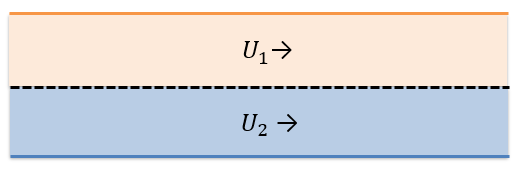
\includegraphics[width=0.7\textwidth]{qg_layers.png} \\
				\end{center}
				\begin{itemize}
					\item[]<2-> $\psi_n = -U_n y$
					\item[]<3-> $q_1 = \frac{1}{\alpha_1}\nabla^2\psi_1 + (\psi_2 - \psi_1) = (U_1 - U_2)y$
					\item[]<3-> $q_2 = \frac{1}{\alpha_2}\nabla^2\psi_2 + (\psi_1 - \psi_2) = (U_2 - U_1)y$
				\end{itemize}
			\end{frame}
			\begin{frame}[t]{Quasigeostrophic Model}
				\begin{align*}
					0 &=\frac{\partial q_1}{\partial t} + D(\psi_1, q_1) \\
					0 &=\frac{\partial q_2}{\partial t} + D(\psi_2, q_2) \\
					D(a, b) &=\frac{\partial a}{\partial x}\frac{\partial b}{\partial y} - \frac{\partial a}{\partial y}\frac{\partial b}{\partial x} \\
				\end{align*}
				\begin{align*}
					\onslide<2->{\mathcal{H} &= \frac12 \iint \sum_{n=1}^2 \left[ \frac{1}{\alpha_n} \vec\nabla \psi_n \cdot \vec\nabla \psi_n + 2C_n(q_n) \right]+ (\psi_1 - \psi_2)^2 \, dA}
				\end{align*}
			\end{frame}

		\subsection{Stability of Zonal Flows}
			\begin{frame}[t]{Second Variation}
				\begin{itemize}
					\item[]<2-> $$\delta^2 \mathcal{H} = \iint \sum_n \left[ \frac{1}{\alpha_n} \vec\nabla\delta\psi_n \cdot \vec\nabla\delta\psi_n + \psi'_n\cdot(\delta q_n)^2 \right]+ (\delta\psi_1 - \delta\psi_2)^2 \, dA$$
					\item[]<3-> $$U_1(U_1 - U_2) = 0$$
					\item[]<3-> $$U_2(U_2 - U_1) = 0$$
				\end{itemize}
			\end{frame}

	\section{References}
		\begin{frame}{References}
			\begin{enumerate}
				\item G. Swaters. "Introduction to Hamiltonian Fluid Dynamics and Stability Theory". Monographs and Surveys in Pure and Applied Mathematics (1999).
				\item  M. E. McIntyre and T. G. Shepherd. "An exact local conservation theorem for finite-amplitude disturbances to non-parallel shear flows, with remarks on Hamiltonian structure and on Arnol’d’s stability theorems". Journal of Fluid Mechanics (1987), vol. 181, pp. 527-565.
				\item T. G. Shepherd. "Symmetries, conservation laws, and Hamiltonian structure in geophysical fluid dynamics". Advances in Geophysics (1990), vol. 32, pp. 287-338.
				\item J. Pedlosky. "Geophysical Fluid Dynamics". Springer Study Edition (1992).
			\end{enumerate}
		\end{frame}

\end{document}
